% !TEX TS-program = pdflatex
% !TEX encoding = UTF-8 Unicode

% This is a simple template for a LaTeX document using the "article" class.
% See "book", "report", "letter" for other types of document.

\documentclass[11pt]{article} % use larger type; default would be 10pt
\usepackage[a4paper, top=20mm, left =20mm, right =20mm ,bottom=20mm ]{geometry}
\usepackage{lineno}
\modulolinenumbers[1]
\journal{TRE}
\usepackage{graphicx}
\usepackage{ulem}
\usepackage{array}
\usepackage{epstopdf}
\usepackage{amstext}
\usepackage[utf8]{inputenc}
\usepackage[english]{babel}
\usepackage{amsfonts}
\usepackage{color}
\usepackage{amssymb}
\usepackage[citecolor=blue,linkcolor=blue,colorlinks=true]{hyperref}
\usepackage{multirow}
\usepackage{amsmath}
%\usepackage{lmodern}
%\usepackage{booktabs}
\usepackage{float}
\usepackage{tabularx}
\usepackage{geometry}
\usepackage{lscape}
\usepackage{longtable}
\usepackage{romannum}
\usepackage{makecell}
\usepackage{adjustbox}
\usepackage{lscape} 
%\usepackage{hyperref}

\usepackage{booktabs}

\usepackage{cleveref}
\usepackage{tablefootnote}
\crefformat{footnote}{#2\footnotemark[#1]#3}
\usepackage{blindtext}
\usepackage{algorithmicx,algpseudocode}
\usepackage[linesnumbered,ruled]{algorithm2e}
\usepackage{amsthm} % add by zhou
\newtheorem{theorem}{Theorem} % add by zhou
 
%\usepackage{longtable}
%\usepackage{natbib} 
%\usepackage[super,square]{natbib} 
\usepackage{longtable} 
\usepackage{float}
\usepackage{footnote}
\renewcommand{\thefootnote}{\arabic{footnote}}
%\pagenumbering{Roman} 
\pagenumbering{arabic} 
\newtheorem{definition}{Definition}
%\newcommand{\red}[1]{\textcolor{red}{#1}}
%%%%%%%%%%%%%%%%%%%%%%%
%% Elsevier bibliography styles
%%%%%%%%%%%%%%%%%%%%%%%
%% To change the style, put a % in front of the second line of the current style and
%% remove the % from the second line of the style you would like to use.
%%%%%%%%%%%%%%%%%%%%%%%
%% Numbered
%\bibliographystyle{model1-num-names}

%% Numbered without titles
%\bibliographystyle{model1a-num-names}

%% Harvard
% \bibliographystyle{model2-names.bst}\biboptions{authoryear}
%% Vancouver numbered
%\usepackage{numcompress}\bibliographystyle{model3-num-names}

%% Vancouver name/year
%\usepackage{numcompress}\bibliographystyle{model4-names}\biboptions{authoryear}

%% APA style
%\bibliographystyle{model5-names}
%\biboptions{authoryear}
%\bibliographystyle{apa}
%% AMA style
%\usepackage{numcompress}\bibliographystyle{model6-num-names}

%% `Elsevier LaTeX' style
%\bibliographystyle{elsarticle-num}
%%%%%%%%%%%%%%%%%%%%%%%
%\bibliographystyle{apalike}
\newlength\mylength
\renewcommand{\baselinestretch}{1.5}
% 
% 
% 
% 
% 
% 
% 
% 
% 
% 
% 
% 
% 

% 
\title{Insights for Auto Port Ranking with LangChain-LLMs}
\author{\textbf{Zehao Qian} \ \ \ \href{mailto:zehao.qian.cn@gmail.com}{zehao.qian.cn@gmail.com}}
\begin{document}
\maketitle
% 
% 
% 
\tableofcontents
% 
% 
% 
% 
\section{Task Schedule Model}
% 
\begin{figure}[H]
    \centering
    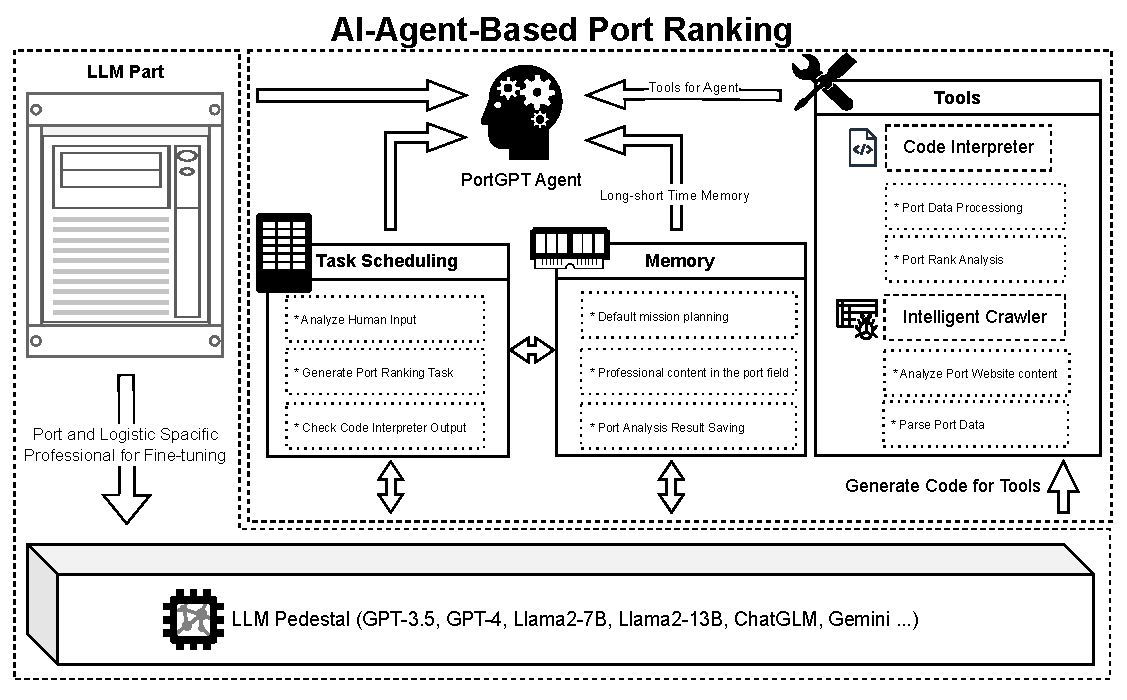
\includegraphics[width=1.0\textwidth]{pic/PortGPT.pdf}
    \caption{PortGPT Conceptual Architecture}
    \label{fig:PortGPT}
\end{figure}
% 
\cite{9458712}
% 
% 
% 
% 
% 
\section{LLM Fine-tuning and Prompt Engineering for Auto Port Ranking}
% 
% 
% 
% 
% 
\section{Port Data Acquisition}
% 
% 
% 
% 
% 
% 
\section{Dealing with Outliers and Missing Values}
% 
% 
% 
% 
% 
% 
% 
% 
% 
\subsection{Outliers}
% 
% 
% 
% 
% 
% 
% 
% 
% 
% 
% 
\subsection{Missing Values}
% 
% 
% 
% 
% 
% 
% 
% 
% 
\paragraph{\textbf{Delete or Impute?} When deciding whether to delete or impute missing data, consider the proportion and pattern of missingness, the nature of the data, the requirements of the analysis method, and the purpose of the study. Deletion is suitable for small proportions of randomly missing data and when it won't introduce bias, while imputation is preferred for large proportions of missing data, non-random missingness, to maintain dataset size and integrity, and to retain critical information. The decision should balance the characteristics of the data, the reasons for missingness, and the objectives of the analysis.}
% 
% 
% 
% 
% 
% 
% 
% 
% 
% 
% 
% 
% 
% 
% 
% 
% 
% 
% 
% 
\bibliographystyle{unsrt}
\bibliography{References}
% 
% 
% 
% 
% 
% 
% 
% 
\end{document}
